\thispagestyle{hoccungpinone}
\pagestyle{hoccungpi}
\everymath{\color{hoccungpi}}
\graphicspath{{../hoccungpi/pic/}}
%\blfootnote{$^{1}$\color{hoccungpi}Đại học Bách Khoa Hà Nội.}
\begingroup
\AddToShipoutPicture*{\put(0,616){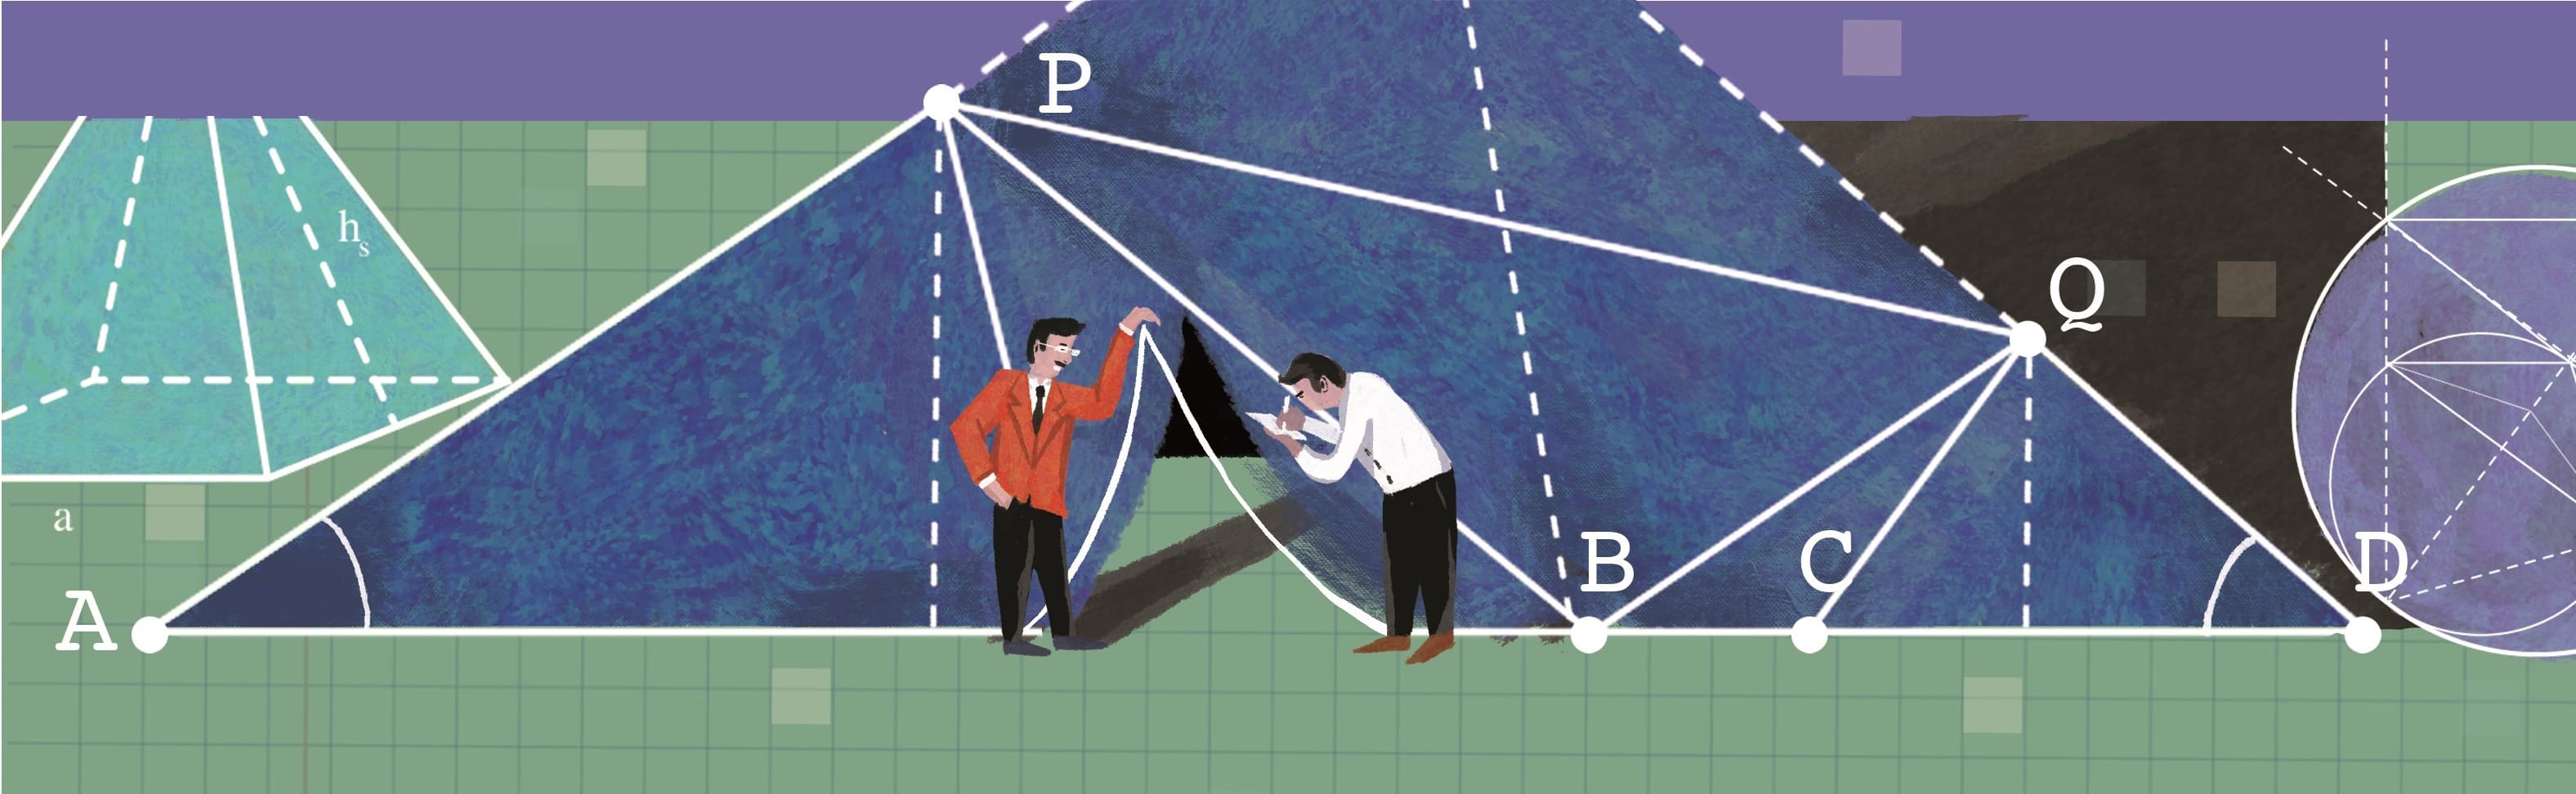
\includegraphics[width=19.3cm]{../bannerhoccungpi}}}
\AddToShipoutPicture*{\put(90,555){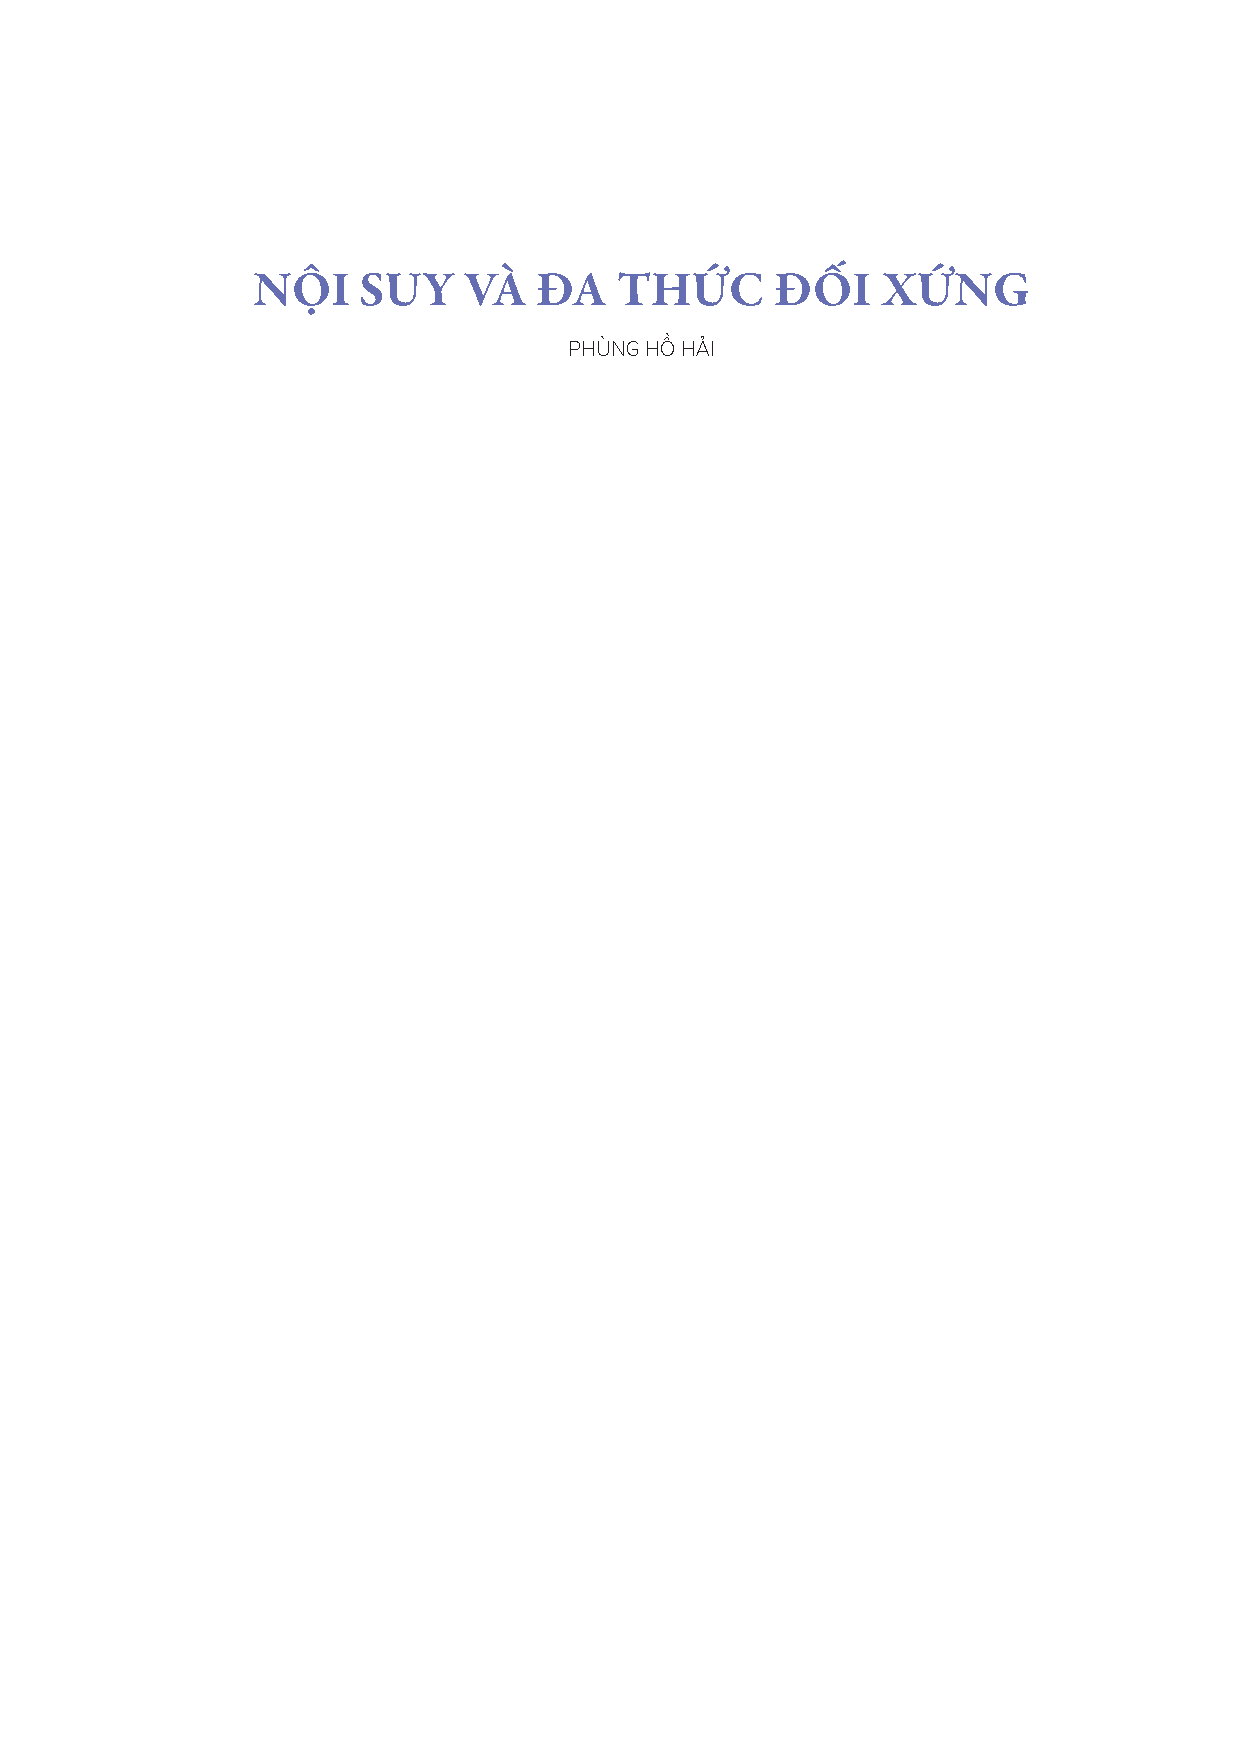
\includegraphics[scale=1]{../tieude.pdf}}}
\centering
\endgroup
\vspace*{155pt}

\begin{multicols}{2}
	$\pmb{1.}$ \textbf{\color{hoccungpi}Đa thức và hàm đa thức} 
	\vskip 0.1cm
	$\pmb{1.1.}$ \textbf{\color{hoccungpi}Đa thức.}
	Đa thức là một biểu thức đại số nhận được một cách hình thức từ các { biến số} và các { hệ số} thông qua các phép tính cộng, trừ và nhân. 
	\vskip 0.1cm
	Các hệ số là phần tử thuộc một tập hợp nào đó, thông thường là một tập hợp số (ví dụ $\mathbb {Z, Q, R, C}$) nhưng cũng có thể là một tập tổng quát hơn mà trên đó đã xác định các phép toán cộng, trừ, nhân. 
	\vskip 0.1cm
	Biến số là các ký tự hình thức (ví dụ $x,y,X,Y,...$) mà ta có thể thay thế chúng bằng những phần tử trong tập hợp chứa các hệ số hoặc một tập hợp lớn hơn mà trên đó cũng xác định các phép toán cộng, trừ và nhân.
	\vskip 0.1cm
	Đa thức một biến có thể được mô tả bằng biểu thức dạng
	\begin{align*}
		P(x)=a_0x^n+a_1x^{n-1}+\ldots+a_n.
	\end{align*}
	Như vậy thông tin về các đa thức một biến bao gồm hai loại: số tự nhiên $n$ được gọi là bậc của nó, ký hiệu là $\deg P(x)$, và các số (nguyên, hữu tỷ, thực hay phức) $a_0,a_1,\ldots, a_n$ -- các hệ số của nó. 
	\begin{tBox}
		Thông tin về đa thức một biến với bậc (không quá) $n$ là một dãy có thứ tự gồm $n+1$ {\em đơn vị thông tin}.
	\end{tBox}
	Dưới đây ta sẽ chỉ xét các { đa thức một biến} với hệ số nằm trong một tập số như $\mathbb{Q, R, C}$. 
	\vskip 0.1cm	
	$\pmb{1.2.}$ \textbf{\color{hoccungpi}Phép chia có dư.}  
	Đối với đa thức hệ số thực ta có thể thực hiện được phép chia có dư, tương tự như đối với các số nguyên. Cho các đa thức $P(x)$ và $Q(x)$ với $Q(x)\neq 0$, khi đó tồn tại duy nhất các đa thức $P_1(x)$ và $R(x)$ với $\deg R(x)<\deg Q(x)$ sao cho
	\begin{align*}
		P(x)= Q(x)P_1(x)+R(x).
	\end{align*}
	Ta nói đa thức $P(x)$ chia hết cho đa thức $Q(x)$ nếu $R(x)=0$.   
	\vskip 0.1cm
	\textbf{\color{hoccungpi}Chú ý}. Ta có thể thay thế điều kiện ``hệ số thực" bởi điều kiện ``hệ số phức" hay ``hệ số hữu tỷ". Nhưng ta không thể áp dụng với điều kiện ``hệ số nguyên". 
	\vskip 0.1cm
	Ví dụ, ta không thể thực hiện được phép chia có dư của đa thức $x^2+1$ cho đa thức $2x$ {trong tập hợp đa thức hệ số nguyên}!
	\vskip 0.1cm
	$\pmb{1.3.}$ \textbf{\color{hoccungpi}Hàm đa thức.}
	Xét các đa thức một biến với hệ số nằm trong một tập số. Khi đó, bằng cách thay thế biến số bằng các giá trị trong tập số đó ta thu được một hàm số. Hàm số thu được bằng cách này gọi là {hàm đa thức}. Chúng thường được mô tả ở dạng
	\begin{align*}
		y=P(x),
	\end{align*}
	trong đó $P(x)$ là một đa thức theo biến $x$.
	\vskip 0.1cm
	{Nguyên lý đồng nhất của Đại số học} nói rằng nếu hai hàm đa thức (trên tập số thực) bằng nhau tại mọi giá trị của biến số thì các đa thức xác định chúng bằng nhau. Nói cách khác, mỗi hàm đa thức được xác định bởi một đa thức duy nhất. 
	\vskip 0.1cm
	Ta chú ý rằng tính đúng đắn của nguyên lý này phụ thuộc vào miền giá trị của biến số (và hệ số). Ví dụ nguyên lý đồng nhất sai nếu xét đa thức trên tập các lớp đồng dư. 
	\vskip 0.1cm	
	$\pmb{1.4.}$ \textbf{\color{hoccungpi}Nghiệm của đa thức.}
	Nghiệm, hay còn gọi là không điểm, của một đa thức $P(x)$ là những giá trị của biến số $x$ mà tại đó $P(x)$ nhận giá trị $0$. Sử dụng phép chia có dư của $P(x)$ cho $x-a$ ta có
	\begin{align*}
		P(x)=(x-a)P_1(x)+P(a).
	\end{align*}
	Như vậy nếu $a$ là nghiệm của $P(x)$ thì $P(x)$ chia hết cho $x-a$. Từ đó ta kết luận một đa thức bậc $n$ { có không quá $n$ nghiệm}.
	\vskip 0.1cm
	{ Định lý cơ bản của Đại số học} khẳng định mọi đa thức với hệ số phức với bậc lớn hoặc bằng $1$ luôn có nghiệm phức. 
	Từ đó suy ra, một đa thức bậc $n\geq 1$ luôn có thể viết được ở dạng
	\begin{align*}
		P(x)=a_0\prod_{i=1}^n(x-x_i), \quad x_i\in\mathbb C.
	\end{align*}
	Chú ý rằng các số (phức) $x_i$ có thể bằng nhau -- trong trường hợp đó ta nói $P(x)$ có {\em nghiệm bội}.
	\begin{tBox}
		Nghiệm bội của một đa thức luôn là nghiệm chung của đa thức đó với đạo hàm của nó. 
	\end{tBox}
	$\pmb{1.5.}$ \textbf{\color{hoccungpi}Các tính chất cơ bản của đa thức dẫn tới nguyên lý nội suy.}
	\vskip 0.1cm
	-- Hai đa thức bằng nhau nếu chúng xác định hai hàm số  bằng nhau (trên các tập số nguyên, hữu tỷ, thực hay phức);
	\vskip 0.1cm
	-- Hai đa thức bằng nhau nếu giá trị chúng bằng nhau tại ``đủ nhiều giá trị của biến số'', phát biểu một cách tương đương là, một đa thức sẽ đồng nhất bằng $0$ nếu nó bằng $0$ tại ``đủ nhiều giá trị của biến số'';
	\vskip 0.1cm
	-- Một đa thức được xác định duy nhất bởi giá trị của nó tại ``đủ nhiều giá trị của biến số'', ``đủ nhiều'' được xác định là nhiều hơn bậc của đa thức. Ví dụ một tập vô hạn luôn là ``đủ nhiều''.
	\vskip 0.1cm
	$\pmb{2.}$ \textbf{\color{hoccungpi}Nội suy Lagrange}
	\vskip 0.1cm
	Bài toán nội duy Lagrange là xác định một đa thức bậc (không quá) $n-1$ từ các giá trị của đa thức tại $n$ vị trí khác nhau.
	\begin{tBox}
		\textbf{\color{hoccungpi}Bài toán nội suy Lagrange.}
		Cho các số $y_1,\ldots, y_n$ và các số phân biệt $x_1,\ldots,x_n$. Xác định đa thức $P(x)$ bậc không quá $n-1$ thỏa mãn:
		\begin{align*}
			P(x_i)=y_i, \text{ với mọi } i=1,2,\ldots, n.
		\end{align*}
	\end{tBox}
	\textbf{\color{hoccungpi}Nhận xét}.
	Nếu tồn tại đa thức $P(x)$ (với bậc không quá $n-1$) nhận giá trị $y_i$ tại điểm $x_i$, 
	$i=1,2,\ldots, n$, thì $P(x)$ là duy nhất. 
	Từ đó suy ra { tính chất tuyến tính} của bài toán nội suy Lagrage:
	\vskip 0.1cm
	-- Giả sử $Q(x)$ là đa thức được xây dựng từ bộ số $(z_1,\ldots, z_n):$
	\begin{align*}
		Q(x_i)=z_i,\quad i=1,\ldots,n,
	\end{align*}
	thì đa thức $P(x)+Q(x)$ được xác định từ bộ số
	\begin{align*}
		(y_1+z_1,\ldots,y_n+z_n).
	\end{align*}
	-- Bộ số $(\lambda y_1,\ldots,\lambda y_n)$ xác định đa thức $\lambda P(x)$ ($\lambda$ là một số bất kỳ).  
	\vskip 0.1cm
	{Trên cơ sở của tính chất tuyến tính, ta sẽ xây dựng đa thức $P(x)$ bắt đầu từ những bộ số $(y_1,\ldots,y_n)$ đơn giản nhất.} 
	\vskip 0.1cm
	-- Nếu tất cả các giá trị $y_i$ đều bằng $0$, ta có $P(x)=0$.
	\vskip 0.1cm  
	-- Nếu $y_1=1, y_2=\ldots=y_n=0$ thì đa thức $P_1(x)$ tương ứng sẽ nhận các giá trị  $x_2,\ldots,x_n$ làm nghiệm. Do $P_1(x)$ có bậc không quá $n-1$ nên  
	\begin{align*}
		P(x)=c(x-x_2)\ldots(x-x_n).
	\end{align*}
	Thay $x=x_1$ ta suy ra
	\begin{align*}
		c=\frac1{(x_1-x_2)\ldots(x_1-x_n)}.
	\end{align*}
	Từ đó
	\begin{align*}
		P_1(x)=\frac{ (x-x_2)\ldots(x-x_n)}{
			(x_1-x_2)\ldots(x_1-x_n)}.
	\end{align*}
	-- Tương tự, với bộ $y_1=\ldots=y_{i-1}=y_{i+1}=\ldots=y_n=0$, $y_i=1$,  đa thức tương ứng là 
	\begin{align*}
		P_i(x) =\prod_{j\neq i}\frac{(x-x_j)}{ (x_i-x_j)}.
	\end{align*}
	Theo nguyên lý tuyến tính nêu trên, ta có lời giải bài toán tổng quát như sau. Đa thức  
	\begin{align*}
		P(x)=\sum_{i=1}^n y_i\prod_{j\neq i}\frac{(x-x_j)}{ (x_i-x_j)} \tag{$1$}
	\end{align*}
	thỏa mãn $P(x_i)=y_i$.
	\vskip 0.1cm
	\textbf{\color{hoccungpi}Chú ý}. Bậc của $P(x)$  có thể bé hơn hẳn $n-1$.
	\vskip 0.1cm
	\textbf{\color{hoccungpi}Bài toán} $\pmb{2.1.}$ Giả sử $A, B$ và $C$ là phần dư của đa thức $P(x)$ khi chia cho $x-a,x-b$ và $x-c$.
		Tìm phần dư của phép chia đa thức đó cho $(x-a)(x-b)(x-c).$
	\vskip 0.1cm
	\textbf{\color{hoccungpi}Bài toán} $\pmb{2.2.}$ Chứng minh rằng nếu $f(x)$ là đa thức bậc nhỏ
		hơn $n$ thì phân thức
		\begin{align*}
			\frac{f(x)}{(x-x_1)(x-x_2)\ldots (x-x_n)}
		\end{align*}
		trong đó $x_1, x_2, \ldots, x_n$ là các giá trị khác nhau, 
		luôn biểu diễn được ở dạng
		\begin{align*}
			\frac{A_1}{x-x_1}+\frac{A_2}{x-x_2}+\ldots +\frac{A_n}{x-x_n}.
		\end{align*}
		với các số $  A_1, A_2,\ldots, A_n$ nào đó.
	\vskip 0.1cm
	\textbf{\color{hoccungpi}Bài toán} $\pmb{2.3.}$ Cho $x_1,\ldots,x_n$ là các số thực phân biệt. Đặt  $g(x):=\prod_{i=1}^n(x-x_i)$. Chứng minh rằng
	\begin{align*}
		\sum_i\frac{x_i^k}{g'(x_i)}= \begin{cases}
			0&\text{ với } k=0,1,\ldots,n-2;\\
			1& \text{ với } k=n-1.
		\end{cases}
	\end{align*}
	\textbf{\color{hoccungpi}Nhận xét.} Trong bài toán trên ta thực sự có các đồng nhất thức, nghĩa là ta có thể coi $x_i$ như là các biến số, tuy nhiên việc chứng minh trực tiếp đồng nhất thức này bằng các biến đổi đại số là rất phức tạp.  
	\vskip 0.1cm
	\textit{Lời giải.} 
	Lấy đạo hàm hai vế của đẳng thức 
	\begin{align*}
			g(x)=\prod_{i=1}^n(x-x_i)  \tag{$2$}
	\end{align*}
	ta thu được:
	\begin{align*}
		g'(x)=\sum_{i=1}^n\prod_{j\neq i}^n(x-x_j).
	\end{align*}  
	Từ đó
	\begin{align*}
		g'(x_i)=\prod_{j\neq i}(x_i-x_j). \tag{$3$}
	\end{align*}
	Áp dụng công thức nội duy Lagrange cho  đa thức $x^k$ ta thu được
	\begin{align*}
		x^k= \sum_{i=1}^nx_i^k\prod_{j\neq i}\frac{(x-x_j)}{ (x_i-x_j)}.
	\end{align*}
	So sánh hệ số của $x^{n-1}$ ở hai vế cho ta các hệ thức cần chứng minh cho $k\leq n-1$.
	\vskip 0.1cm
	\textbf{\color{hoccungpi}Bài toán} $\pmb{2.4.}$ Tính 
	\begin{align*}
		h_{k}:=\sum_i\frac{x_i^{n+k-1}}{g'(x_i)},
	\end{align*}
	với $k=1,2,3.$
	\vskip 0.1cm 
	\textit{Lời giải.} 
	Xét công thức Viète 
	\begin{align*}
		g(x)\!=\!\prod_{i=1}^n(x\!-\!x_i)\!=\!x^{n}\!-\!e_1x^n\!+\!\ldots\!+\!(\!-\!1)^{n}e_{n}.
	\end{align*}
	Các hệ số $e_i$ là các { đa thức đối xứng cơ bản} theo
	các biến $x_1,\ldots,x_n$. 
	\vskip 0.1cm
	Nhân theo vế đẳng thức $g(x_i)=0$ với $x_i^{k}$ ta thu được
	\begin{align*}
		x_i^{n+k}-e_1x_i^{n+k-1}+\ldots+(-1)^{n}e_{n}
		x_i^{k}=0.
	\end{align*}	
	{ Chia theo vế cho  $ \prod_{j\neq i}(x_i-x_j)$}
	và lấy tổng theo $i$, ta thu được 
	\begin{align*}
		h_{k+1}-e_1h_{k}+\ldots+(-1)^{n}e_{n}h_{k+1-n}=0,
	\end{align*}
	với quy ước { $h_0=1$ và $h_k=0$ nếu $k<0$.} 
	Công thức trên cho phép ta tính các đa thức $h_k$. 
	Cụ thể ta có: 
	\begin{align*}
		h_1=e_1&=\sum_i x_i\\
		h_2=e_1h_1-e_2&=\sum_{i\leq j}x_ix_j\\
		h_3=e_1h_2-e_2h_1+e_3&=\sum_{i\leq j\leq k}x_ix_jx_k.
	\end{align*}
	\textbf{\color{hoccungpi}Nhận xét}. Trong lời giải trên ta sử dụng hai kỹ thuật. Thứ nhất là thế $x=x_i$ vào $g(x)$ để thu được một hệ thức giữa  $x_i$ và các hệ số $e_j$. Thứ hai là nhân hệ thức đó theo các {trọng số}. 
	\vskip 0.1cm
	\textbf{\color{hoccungpi}Bài toán} $\pmb{2.5.}$  Chứng minh công thức tổng quát sau với mọi $k=4,5, \ldots$
	\begin{align*}
		h_k=\sum_{i_1\leq i_2\leq\ldots\leq i_k}x_{i_1}x_{i_2}\ldots x_{i_k}.
	\end{align*}
	Các đa thức $h_k$ được gọi là { \em đa thức đối xứng toàn phần} theo các biến $x_1,\ldots,x_n$.
	\vskip 0.1cm
	$\pmb{2.1.}$ \textbf{\color{hoccungpi}Hệ số của đa thức nhận được từ công thức nội suy Lagrange.}
	Trong bài tập $2.1$ ta đã sử dụng phương pháp so sánh hệ số trong công thức nội suy Lagrange. Một câu hỏi tự nhiên là: { có thể mô tả cụ thể được các hệ số của $P(x)$ từ các giá trị $y_i$ và $x_i$ hay không?}
	\vskip 0.1cm
	Từ đẳng thức
	\begin{align*}
		P(x)&= a_0x^{n-1}+a_1x^{n-2}+\ldots+a_{n-1} \\
		&= \sum_{i=1}^n y_i \frac{\prod_{j\neq i}^n(x-x_i)}{g'(x_i)}, \tag{$6$}
	\end{align*}
	so sánh hệ số ta thu được:
	\begin{align*}
		a_0= \sum_{i=1}^n 
		\frac{ y_i}{g'(x_i)} ,
	\end{align*}
	và 
	\begin{align*}
		a_1= \sum_{i=1}^n
		\frac{y_i (x_i-e_1)}{g'(x_i)}=
		\sum_{i=1}^n \frac{y_i  x_i}{g'(x_i)}-a_0e_1.
	\end{align*}
	\textbf{\color{hoccungpi}Bài toán} $\pmb{2.6.}$
	Đặt
	\begin{align*}
		b_k:=\sum_i\frac{y_i x_i^k}{g'(x_i)}.
	\end{align*}
	Chứng minh rằng các hệ số của đa thức $P(x)$ được tính bởi công thức
	\begin{align*}
		a_k=\sum_{j=0}^k(-1)^i e_jb_{k-j}.
	\end{align*}
	$\pmb{2.2.}$ \textbf{\color{hoccungpi}Đạo hàm bậc hai.} Trong các tính toán ở trên ta đã sử dụng các giá trị của đạo hàm bậc nhất của $g'(x)$. Vậy đạo hàm bậc hai có ý nghĩa gì? 
	\vskip 0.1cm
	\textbf{\color{hoccungpi}Bài toán} $\pmb{2.7.}$ Giả thiết rằng các số $x_i$ phân biệt, khi đó $g''(x_i)=0$ khi và chỉ khi
	\begin{align*}
		  \sum
		_{j\neq i}^n\frac1{x_i-x_j}=0.
	\end{align*}
	\textit{Lời giải.} 
	Tính đạo hàm hai lần của $g(x)$. Ta có
	\begin{align*}
		g''(x)=\sum_{k\neq  j}\prod_{i\neq k,j}(x-x_i)= \sum_{k\neq j}\frac{g(x)}{(x-x_k)(x-x_j)}.
	\end{align*}
	Từ đó ta có, với mỗi $1\leq i\leq n$: 
	\begin{align*}
		g''(x_i)=2\prod_{j\neq i}(x_i-x_j)\sum_{j\neq i}^n\frac1{x_i-x_j}.
	\end{align*}
	Vậy $g''(x_i)=0$ khi và chỉ khi
	\begin{align*}
		\sum_{j\neq i}\frac1{x_i-x_j}=0.
	\end{align*}  
	\textbf{\color{hoccungpi}Bài toán} $\pmb{2.8.}$
	Cho các số $0=x_0<x_1<\ldots<x_{n+1}=1$ thỏa mãn
	\begin{align*}
		\sum_{j=0,j\neq i}^{n+1}\frac1{x_i-x_j}=0,
	\end{align*}
	với mọi $i=1,2,\ldots,n$. Chứng minh rằng với mọi $i$, $x_i=1-x_{n+1-i}$.
	\vskip 0.1cm 
	$\pmb{3.}$ \textbf{\color{hoccungpi}Hàm sinh}
	\vskip 0.1cm
	Hàm sinh là một  công cụ dùng để phát biểu nhiều vấn đề của số học hay tổ hợp theo ngôn ngữ đại số, trên cơ sở đó sử dụng các phương pháp đại số (và giải tích) để giải quyết vấn đề. 
	\vskip 0.1cm
	Để xác định, hay tìm hiểu tính chất của một dãy số $a_0,a_1,\ldots$, thay vì nghiên cứu từng số hạng riêng rẽ, người ta tập hợp tất cả chúng trong một { \em tổng hình thức} hay một chuỗi lũy thừa:
	\begin{align*}
		A(x):=a_0+a_1 x+\ldots+ a_nx^n+\ldots.
	\end{align*}
	Nếu dãy đã cho hữu hạn, thì $A(x)$ là một đa thức. Như vậy các chuỗi lũy thừa có thể coi như một \textit{ khái niệm mở rộng của đa thức}.
	\vskip 0.1cm
	Tương tự như với đa thức, ta có thể quy ước các phép tính cộng, trừ hay nhân các hàm sinh.   
	\vskip 0.1cm
	Phép cộng và trừ được thực hiện theo thành phần (nghĩa là tương ứng với phép cộng, trừ hai dãy số).
	\vskip 0.1cm
	Phép nhân được thực hiện tương tự nhân đa thức. Với hai hàm sinh
	\begin{align*}
		A(t)=\sum_0^\infty a_ix^i,\quad B(t)=\sum_0^\infty b_i x^i,
	\end{align*}
	tích của chúng là hàm sinh $C(t)=\sum_0^\infty c_ix^i$, với các hệ số $c_i$ cho bởi công thức
	\begin{align*}
		c_i=\sum_{j=0}^i a_jb_{i-j}.
	\end{align*}
	$\pmb{3.1.}$ \textbf{\color{hoccungpi}Ví dụ.}
	\vskip 0.1cm
	-- Với
	\begin{align*}
		A(x)&=1-x,\\
		B(x)&=1+x+x^2+\ldots+x^n+\ldots
	\end{align*}
	ta có 
	\begin{align*}
		A(x)\cdot B(x)=1.
	\end{align*}
	Nghĩa là ta có đẳng thức
	\begin{align*}
		1+x+x^2+\ldots+x^n+\ldots=\frac 1{1-x}.
	\end{align*}
	Từ đó ta cũng có
	\begin{align*}
		B(x)^2&=1+2x+3x^2+\ldots+(n+1)x^n+\ldots\\
		&=\frac1{1-2x+x^2}.
	\end{align*}
	-- Hàm sinh cho dãy  các đa thức đối xứng cơ bản của $x_1,x_2,\ldots,x_n$ là: 
	\begin{align*}
		E(x)=1+e_1x+\ldots +e_nx^n=\prod_{i=1}^n (1+x_ix).
	\end{align*}   
	Xét hệ thức
	\begin{align*}
		&\frac 1{E(-x)}=\prod_i \frac 1{1-x_ix}\\
		=&\prod_i (1+x_i x+\ldots+x_i^nx^n+\ldots)\nonumber \\
		=& 1+h_1x+h_2x^2+\ldots+h_nx^n+\ldots  \tag{$7$}
	\end{align*} 
	\begin{align*}
		h_r=\sum_{i_1\leq\ldots\leq i_r}x_{i_1}\cdots x_{i_r}.
	\end{align*}
	-- Các đa thức  $h_r$ là các { đa thức đối xứng toàn phần} theo  $x_1,\ldots, x_n$. 
	Từ trên ta rút ra hệ thức sau giữa các đa thức $e_i$ và $h_i$:
	\begin{align*}
		&h_k-e_1h_{k-1}+\ldots+(-1)^ke_k=0,\\
		&\text{ với mọi }   1\leq k\leq n;\\
		&h_k-e_1h_{k-1}+\ldots+(-1)^ne_n h_{k-n}=0,\\
		&\text{ với mọi }    k\geq n.
	\end{align*}
	$\pmb{3.2.}$ \textbf{\color{hoccungpi}Đạo hàm của hàm sinh.}
	Ngoài các phép toán đại số nêu trên, ưu thế quan trọng của hàm sinh là ta có thể thực hiện phép {\em đạo hàm} trên chúng. 
	\vskip 0.1cm
	Nếu $A(x)=\sum a_nx^n$ thì 
	\begin{align*}
		A'(x):=\sum_{n=0}^\infty  (n+1)a_{n+1}x^n.
	\end{align*} 
	Bài tập dưới đây cho thấy hai phép toán định nghĩa như trên thỏa mãn các tính chất quen biết của phép toán đạo hàm và tích phân.
	\vskip 0.1cm
	\textbf{\color{hoccungpi}Bài toán} $\pmb{3.1.}$ Kiểm tra các hệ thức sau:
		\begin{align*}
			(A(t)\cdot B(t))'&=A(t)'\cdot B(t)+A(t)\cdot B(t)'\\
			\left(\frac 1{A(t)}\right)'&=-\frac{A(t)'}{A(t)^2}		
		\end{align*}
	\textbf{\color{hoccungpi}Bài toán} $\pmb{3.2.}$ Hàm mũ $\exp$ và hàm logarit $\ln$ được định nghĩa như sau:
	\begin{align*}
		\exp(x)=1+x+\ldots+\frac{x^n}{n!}+\ldots \tag{$8$}\\
		\ln(1\!+\!x)\!=\!x\!-\!\frac{x^2}2\!+\!\ldots\!+\!(\!-\!1)^n\frac{x^n}n\!+\!\ldots\! \tag{$9$}
	\end{align*}
	Chứng minh rằng
	\vskip 0.1cm
	-- $\exp(x)'=\exp(x)$, $\ln(x)'=\frac1{1+x}$;
	\vskip 0.1cm
	-- với mỗi hàm sinh $A(x)$ với hệ số đầu tiên bằng $0$, nghĩa là $A(0)=0$, thì $\exp(A(x))$ cũng là một hàm sinh;
	\vskip 0.1cm
	-- với mỗi hàm sinh $A(x)$với hệ số đầu tiên bằng $0$, nghĩa là $A(0)=1$, thì $\ln(A(x))$ cũng là một hàm sinh;
	\vskip 0.1cm
	-- $\exp(\ln(1+x))=1+x$, $\ln(\exp(x))=x$.
	\vskip 0.1cm
	$\pmb{4.}$ \textbf{\color{hoccungpi}Đa thức đối xứng} 
	\vskip 0.1cm
	Đa thức theo $n$ biến $x_1,x_2,\ldots,x_n$ được gọi là đối xứng nếu nó không thay đổi khi ta hoán vị các biến. Ta đã làm quen với các đa thức đối xứng sau: 
	\vskip 0.1cm
	-- Đa thức đối xứng cơ bản
	\begin{align*}
		e_r=\sum_{i_1<i_2<\ldots<i_r}x_{i_1}x_{i_2}\ldots x_{i_r},\quad r=1,2,\ldots, n.
	\end{align*}
	-- Đa thức đối xứng toàn phần
	\begin{align*}
		h _r=\sum_{i_1\le i_2\le \ldots \le i_r}x_{i_1}x_{i_2}\ldots x_{i_r},\quad r=1,2,\ldots,n.
	\end{align*}
	-- Ngoài ra ta còn đó tổng lũy thừa 
	\begin{align*}
		p_r=\sum_i x_i^r, r=1,2,\ldots
	\end{align*}
	Ứng với mỗi loại đa thức đối xứng ở trên ta sẽ xét hàm sinh của nó. Như ở phần trên ta có
	\begin{align*}
		E(x)&=\sum_{i=0}^n e_ix^i=\prod(1+x_ix),\\
		H(x)&=\sum_{i=0}^\infty h_i x^i=\prod\frac1{1-x_i x},\\
		P(x)&= \sum_{i=0}^\infty p_{i+1} x^{i}=\sum_{i=1}^n \frac {x_i}{1-x_i x}.
	\end{align*}	
	Từ hệ thức ($7$) ta có  $E(-x)\cdot H(x)=1$.
	\vskip 0.1cm
	Mặt khác, xét đạo hàm của $\ln E(x)$ ta có
	\begin{align*}
		\ln(E(x))'&=\frac{E'(x)}{E(x)}= \sum_i\ln\left({1+x_i x}\right)'\\
		&=\sum_i\frac{x_i}{1+x_i x}.
	\end{align*}
	Từ đó ta suy ra hệ thức:
	\begin{align*}
		E'(x)=E(x)\cdot P(-x).
	\end{align*}
	Đây chính là { hệ thức Newton} đối với các tổng lũy thừa.   
	So sánh hệ số của $x^{k}$ ở hai vế ta có.
	\vskip 0.1cm
	-- Với $0\leq k\leq n-1$:
	\begin{align*}
		(k+1)e_{k+1}=&e_kp_1-e_{k-1}p_2+\ldots\\
		&+(-1)^{k-1} e_1p_k+(-1)^{k}p_{k+1}
	\end{align*}
	hay là 
	\begin{align*}
		p_{k+1}=&e_1p_k+\ldots+(-1)^{k-1}e_kp_1\\
		&+(-1)^{k}(k+1)e_{k+1}.
	\end{align*}
	-- Với $k\geq n$:
	\begin{align*}
		0=&e_np_{k+1-n}-e_{n-1}p_{k+2-n}+\ldots\\
		&+(-1)^{n-1} e_1p_k+(-1)^{n}p_{k+1}
	\end{align*}
	hay là 
	\begin{align*}
		p_{k+1}=e_1p_k+\ldots+(-1)^{n-1}e_np_{k+1-n}.
	\end{align*}
	\textbf{\color{hoccungpi}Bài toán} $\pmb{4.1.}$ Chứng minh trực tiếp hệ thức Newton. 
			(Với trường hợp $k\geq n$, sử dụng phương pháp trong lời giải bài toán $2.4$. Với trường hợp $k<n$, sử dụng quy nạp theo số biến).
	\vskip 0.1cm
	\textbf{\color{hoccungpi}Bài toán} $\pmb{4.2.}$  Giả thiết $x_1,\ldots,x_n$ là các nghiệm (thực hoặc phức) của đa thức
	\begin{align*}
		x^n-{m\choose 1}x^{n-1}+\ldots+(-1)^n{m\choose n}
	\end{align*}
	với $m$ là số tự nhiên bất kỳ.
	Tính tổng
	\begin{align*}
		\sum x_i^k,\quad k=1,2,\ldots,n.
	\end{align*} 
	\textbf{\color{hoccungpi}Bài toán} $\pmb{4.3.}$
	Cho các số thực $a_1,\ldots,a_n$ và các số nguyên dương $b_1,\ldots,b_n$. Giả thiết tồn tại đa thức $f(x)$ sao cho:
	\begin{align*}
		(1-x)^nf(x)=1+\sum_i a_ix^{b_i}
	\end{align*}
	Tính $f(1)$ qua $b_i$ và $n$.
	\vskip 0.1cm
	$\pmb{5.}$ \textbf{\color{hoccungpi}Dãy cho bởi hệ thức truy hồi}
	\vskip 0.1cm
	Cho trước các số $e_1,e_2,\ldots,e_n$. Ta xét dãy vô hạn $(a_k)$, $k=0,1,\ldots$ các số thỏa mãn { hệ thức truy hồi}
	\begin{align*}
		&a_{n\!+\!k}\!=\!e_1a_{n\!+\!k\!-\!1}\!-\!e_2a_{n\!+\!k\!-\!2}\!+\!\ldots\!+\!(\!-\!1)^{n}e_na_k,\\
		&\quad k=0, 1,\ldots
	\end{align*}
	với các giá trị  $a_0,a_1,\ldots,a_{n-1}$ cho trước. 
	\vskip 0.1cm	
	-- Dãy $(a_n)$ được xác định duy nhất bởi hệ thức trên, và các số hạng
			$a_0, a_1,\ldots, a_{n-1}$ được gọi là {  điều kiện ban đầu}.
	\vskip 0.1cm  
	--	Bài toán xác định một dãy số thỏa mãn hệ thức truy hồi như trên còn được gọi là bài toán {\em giải phương trình sai phân}. 
	\vskip 0.1cm
	-- Đa thức 
	\begin{align*}
		g(x)=x^n-e_1x^{n-1}+\ldots+(-1)^n e_n
	\end{align*}
	được gọi là { đa thức đặc trưng} của phương trình trên.
	\vskip 0.1cm
	$\pmb{5.1.}$ \textbf{\color{hoccungpi}Nghiệm tổng quát.} 
	Việc xác định dãy từ hệ thức truy hồi và điều kiện ban đầu được thực hiện theo hai bước.
	\vskip 0.1cm
	--  Xác định tất cả các dãy thỏa mãn hệ thức truy hồi -- đây gọi là { các nghiệm tổng quát} của bài toán;
	\vskip 0.1cm
	--  Kết hợp với điều kiện ban đầu để xác định dãy cần tìm trong số các dãy ở trên -- đây gọi là { nghiệm riêng} của bài toán.
	\vskip 0.1cm	
	Gọi $t$ là một nghiệm của $g(x)$. Khi đó dãy $(\lambda t^k)_{k\geq 0}$
	thỏa mãn hệ thức truy hồi  ở trên, với mọi số $\lambda$.
	\vskip 0.1cm	
	Giả thiết $g(x)$ có $n$ { nghiệm phân biệt} $x_1,\ldots,x_n$ (có thể là nghiệm phức). Khi đó với mọi bộ số $\lambda_1,\ldots, \lambda_n$, dãy $(a_k)$ cho bởi
	\begin{align*}
		a_k=\sum_{i=1}^n \lambda_i x_i^k
	\end{align*}
	thỏa mãn hệ thức truy hồi ở trên.
	\vskip 0.1cm	
	$\pmb{5.2.}$ \textbf{\color{hoccungpi}Nghiệm riêng.}
	Các hệ số $\lambda_i$ được tính cụ thể thông qua điều kiện ban đầu $a_0,\ldots,a_{n-1}$ bằng cách giải hệ phương trình
	\begin{align*}
		\label{ini-cond}\sum \lambda_i x_i^k=a_k,\quad k=0,1,\ldots,n-1. \tag{$10$}
	\end{align*}
	Chúng ta sẽ mô tả nghiệm $(\lambda_1,\ldots,\lambda_n)$ của hệ này nhờ bài toán nội suy. 
	Cụ thể, ta tìm $\lambda_i$ ở dạng
	\begin{align*}
		\lambda_i=\frac{P(x_i)}{g'(x_i)},
	\end{align*}
	với $P(x_i)$ là một đa thức bậc $n-1$:
	\begin{align*}
		P(x)\!=\!b_0x^{n\!-\!1}\!-\!b_1x^{n\!-\!2}\!+\!\ldots\!+\!(\!-\!1)^{n\!-\!1}b_{n\!-\!1}.
	\end{align*}
	Nghĩa là
	\begin{align*}
		a_k\!=\!\sum_iP(x_i)\frac{x_i^k}{g'(x_i)},\,\,\, \text{ với } k=0,1,\ldots,n\!-\!1.
	\end{align*}
	Thế giá trị của $P(x_i)$ và sử dụng kết quả của bài tập $2.3$ ta có
	\begin{align*}
		a_k&=\sum_{j=0}^{n-1}(-1)^jb_j
		{\sum_i
			\frac{x_i^{n-1-j+k}}{g'(x_i)}}\\
		&=\sum_{j=0}^{n-1}(-1)^jb_j{ h_{k-j}}.
	\end{align*}
	Vậy, sử dụng hệ thức ($5$) giữa $e_i$ và $h_j$ ta thu được: 
	\begin{align*}
		b_k=\sum_{j=0}^k(-1)^ja_je_{k-j}. \tag{$11$}
	\end{align*}
	Cụ thể
	\begin{align*}
		b_0&=a_0\\
		b_1&=a_0e_1-a_1\\
		b_2&=a_0e_2-a_1e_1+a_2\\
		\dots&\\
		b_{n\!-\!1}&=a_0e_{n\!-\!1}\!-\!a_1e_{n\!-\!2}\!+\!\ldots\!+\!(\!-\!1)^{n\!-\!1}a_{n\!-\!1}.
	\end{align*}
	Ta cũng có cách mô tả khác cho $P(x)$ như sau:
	\begin{align*}
		P(x)=&a_0(x^{n\!-\!1}\!-\!e_1x^{n\!-\!2}\!+\!\ldots\!+\!(\!-\!1)^{n\!-\!1}e_{n\!-\!1})\\
		&\!+\!a_1(x^{n\!-\!2}\!-\!e_1x^{n\!-\!3}\!+\!\ldots\!+\!(\!-\!1)^{n\!-\!2}e_{n\!-\!2})\\
		&+
		\ldots+a_{n-1}.
	\end{align*}
	\textbf{\color{hoccungpi}Bài toán} $\pmb{5.1.}$ Chứng minh rằng với mỗi $k=1,2,\ldots,n-1$, giá trị của đa thức
	\begin{align*}
		c_k(x):=(-1)^k(x^k-e_1x^{k-1}+\ldots+(-1)^ke_k)
	\end{align*}
	tại $x_i$ là đa thức đối xứng thứ $k$ theo $n-1$ biến $x_j$,  $j\neq i$.
	\vskip 0.1cm	
	Từ bài toán $5.1$ ta có công thức sau cho các hệ số $\lambda_i$:
	\begin{align*}
		\lambda_i=\frac{1}{g'(x_i)}\sum_{k=0}^{n-1}(-1)^ka_ke_{n-k-1, (x_i=0)}.
	\end{align*}
	Trong đó $e_{k,(x_i=0)}$ ký hiệu đa thức đối xứng thứ $k$ theo các biến $x_j,j\neq i$ (nhận được từ $e_k$ bằng cách cho $x_i=0$). Ví dụ:
	\vskip 0.1cm
	-- $n=2$. Ta có 
	\begin{align*}
		\lambda_1= \frac{a_1-a_0x_2}{x_1-x_2},\quad 
		\lambda_2=\frac{a_1-a_0x_1}{x_2-x_1}.
	\end{align*}
	-- $n=3$. Ta có
	\begin{align*}
		\lambda_i&=&\frac{a_0x_jx_k-a_1(x_j+x_k)+a_2}{(x_i-x_j)(x_i-x_k)}, 
	\end{align*}
	trong đó $(i,j,k)$ là một hoán vị của $(1,2,3)$.	
	\vskip 0.1cm
	$\pmb{5.3.}$ \textbf{\color{hoccungpi}Sử dụng hàm sinh.}  
	Ta có thể dùng hàm sinh để thu được công thức ($11$) cho các hệ số của $P(x)$  như sau.
	Xét hàm sinh của dãy $(a_n)_{n\geq 0}$
	\begin{align*}
		A(x)=\sum_{n=0}^\infty a_n x^n.
	\end{align*}
	Xét đa thức
	\begin{align*}
		G(x)\!:=\!{ x^ng(1/x)}&=\!1\!-\!e_1x\!+\!\ldots\!+\!(\!-\!1)^n e_n x^n\\
		&=\!\prod_i(1-x_i x).
	\end{align*}
	Hệ thức truy hồi suy ra:
	\begin{align*}
		A(x)\cdot G(x)=B(x),
	\end{align*}
	với đa thức $B(x)=b_0+b_1x+\ldots+b_{n-1}x^{n-1}$ được cho bởi
	\begin{align*}
		b_k=\sum_{j=0}^k (-1)^j a_{j}e_{k-j}.
	\end{align*}
	Vậy
	\begin{align*}
		A(x)= \frac{B(x)}{G(x)}.
	\end{align*}
	Nhận xét rằng công thức trên cho hàm $A(x)$ đúng cả khi các giá trị $x_i$ không phân biệt. 
	\vskip 0.1cm	
	Nếu các giá trị $x_i$ là phân biệt, do $\deg B(x)\leq n-1$, theo bài toán $2.2$ ta có khai triển
	\begin{align*}
		\frac{B(x)}{G(x)}=\sum_i\frac{\lambda_i}{1-x_i x}.
	\end{align*}
	Nhân cả hai vế hệ thức trên với $(1-x_ix)$ và thay $x=1/x_i$ ta thu được
	\begin{align*}
		\lambda_i=\frac{B(1/x_i)}{\prod_{j\neq i}(1-x_j/x_i)} = 
		\frac{x_i^{n-1}B(x_i)}{g'(x_i)}.
	\end{align*}
	Dễ thấy { $x^{n-1}B(1/x)=P(x).$}
	\vskip 0.1cm	
	\textbf{\color{hoccungpi}Bài toán} $\pmb{5.2.}$ Ký hiệu $x_n$ là số các số $n$ chữ số trong đó chỉ có các chữ số $2,3,5,7$ xuất hiện và $5$ không đứng ngay sau $2$. Chứng minh rằng với mọi $r\geq 1$ và $m\geq2$, ta luôn có $x_{rm-1}$ chia hết cho $x_{m-1}$.
	\vskip 0.1cm
	\textbf{\color{hoccungpi}Bài toán} $\pmb{5.3.}$ Xét dãy $(f_n)$:
	\begin{align*}
		f_n=a f_{n-1}+b f_{n-2}, \quad f_0=c, f_1=d
	\end{align*}
	và $p$ là số nguyên tố, $p>2$. Chứng minh rằng, theo modulo $p$:
	\vskip 0.1cm
	-- nếu $a^2+4b$ chính phương thì $f_p\equiv d$;
	\vskip 0.1cm 
	-- nếu $a^2+4b$ không chính phương thì $f_p\equiv ca-d$;
	\vskip 0.1cm
	--nếu $a^2+4b\equiv 0$ thì $2f_p\equiv ac$.
	\vskip 0.1cm
	\textbf{\color{hoccungpi}Bài toán} $\pmb{5.4.}$  Cho $x_0=4$, $x_1=x_2=0$, $x_3=3$,
	\begin{align*}
		x_{n+4}=x_{n+1}+x_n.
	\end{align*}
	Chứng minh rằng $x_p$ chia hết $p$ với mọi $p$ nguyên tố.
	\vskip 0.1cm	
	$\pmb{6.}$ \textbf{\color{hoccungpi}Lời giải và gợi ý}
	\vskip 0.1cm
	$\pmb{6.1.}$ \textbf{\color{hoccungpi}Lời giải bài} $\pmb{2.5.}$ Sử dụng hệ thức ($5$) và các kết quả trong ví dụ $3.1$. 
	\vskip 0.1cm
	$\pmb{6.2.}$ \textbf{\color{hoccungpi}Lời giải bài} $\pmb{2.6.}$
	Từ hệ thức ($6$) ta có
	\begin{align*}
		P(x)=&a_0x^{n-1}+a_1x^{n-2}+\ldots+a_{n-1}\\
		=&g(x)\sum_i \frac{y_i}{g'(x_i)(x-x_i)}.
	\end{align*}
	Thay $x$ bằng $1/x$ trong hệ thức trên và nhân theo vế với $x^{n-1}$ ta thu được
	\begin{align*}
		x^nP(1/x)&=\prod_i(1-x_i x)\sum_i\frac{y_i}{g'(x_i)(1-x_i x)}\\
		&=E(-x) \sum_{k=0}^\infty b_i x^k.
	\end{align*}
	Hay là
	\begin{align*}
		a_0+a_1 x+\ldots + a_{n-1}x^{n-1}= 
		E(-x) \sum_{k=0}^\infty b_i x^k.
	\end{align*}
	Từ đó ta có điều phải chứng minh. 
	\vskip 0.1cm	
	$\pmb{6.3.}$ \textbf{\color{hoccungpi}Lời giải bài} $\pmb{4.3.}$
	Cho $x=1$ ta thu được 
	\begin{align*}
			\sum_i a_i=-1. \tag{$12$}
	\end{align*}
	Đạo hàm cả hai vế rồi cho $x=1$ ta thu được
	\begin{align*}
		\sum_i a_ib_i=0. \tag{$13$}
	\end{align*}
	Đạo hàm hai lần cả hai vế rồi cho $x=1$ ta thu được
	$ \sum_i a_ib_i(b_i-1)=0$.
	Kết hợp với ($13$) ta thu được
	\begin{align*}
		\sum_i a_ib_i^2 =0. \tag{$14$} 
	\end{align*}
	Tương tự ta thu được các đẳng thức với $k=2,3,\ldots, n-1$:
	\begin{align*}
		\sum_i a_ib_i^k =0. \tag{$15$}
	\end{align*}
	Đạo hàm $n$ lần cả hai vế rồi cho $x=1$ ta thu được
	\begin{align*}
		(-1)^n n! f(1)=\sum_ia_i b_i^n  .
	\end{align*}
	Vậy bài toán đưa về  tính tổng $\sum_i a_ib_i^n $ theo các số $n$ và $b_i$, biết rằng 
	\begin{align*}
		\left\{\begin{array}{rcl}
			\sum_i a_i&=&-1 \\
			\sum_i a_ib_i&=&0\\
			\multicolumn{3}{c}{\dotfill }\\
			\sum_i a_i b_i^{n-1}&=&0.\end{array}\right.
	\end{align*}
	Xét $P(x)=\prod(x-b_i)=x^n-e_1x^{n-1}+\ldots+(-1)^ne_n$. 
	Nhân theo vế với $a_i$  ta có
	\begin{align*}
		a_ib_i^n-a_ie_1b_i^{n-1}+\ldots+(-1)^na_ie_n=0.
	\end{align*}
	Lấy tổng theo $i$ suy ra
	\begin{align*}
		\sum_i a_ib_i^n=(-1)^n\prod_i b_i.
	\end{align*}
\end{multicols}